\documentclass{article}
\usepackage[utf8]{inputenc}
\usepackage{hyperref}
\usepackage{graphicx}
\title{Journal 3}
\author{Riyam ALbazrkan }
\date{November 8 2022}


\begin{document}

\maketitle

\section{survey paper learning/process}
At the beginning doing this journal now seems so accurate although it fells like travelling back in time .
So Far this process is very complex and didn't have a clear vision till a week ago.
At the beginning i had zero idea of what i want to do , then found an interesting paper that somehow drew some clear path which was the start of the road of researching in this particular topic
this is the link to the article.
\newline
\url{https://www.hindawi.com/journals/cin/2022/2926241/}
Then afterwords i switched to Text Summrization to be my topic that i should stick with till the end of this semester,but meanwhile searching and reading i found myself drifting away and not focousing on what i should do actually .
but all that leads to consumming alot of time and working hard on deleviring on time .
I alwasys beleive in the process (just give things time ) and everything will workout perfectlly (hop11fully).
So now i am back on track working on navigating my way through Augmentaed reialiy usage .
\newpage
\section{Creative Reading}
In this part i will say that not much of the articales are modern exepet of a very usefull book that is two years old which makes it very convinet ,and also focuses on what i am looking for so actually it is a very good reference.
Also the papers are not open to public yet in order to read them you have to purchaes the book 
but these are some main points about 4 of the articals inside this book
\newline
\begin{itemize}
    \item Museums in 21st century: Implementing augmented reality and virtual reality technologies alongside social Media's\cite{kargas2020reinventing} :
    \newline
    This paper is cited by 11 
    The Paper introduced a novel term (industry4.0) which seems to be  promising for digitizing museums , that was the hook effect that makes you eager to learn more and discover.
    Also it linked everything with social media i guess it is a very good aspect to attract readers even if they are not interested in this field or if they don't have a background in computer science but for sure they do use social media on a daily bases .
    additional good point is the number of the examples that this paper provided.
    
    \item Challenges of Mobile Augmented Reality in Museums and Art Galleries for Visitors Suffering From Vision, Speech, and Learning Disabilities\cite{kunjir2020challenges} :
    \newline
    This article  cited by 1 
    This is considered to be the lowest cited paper although is focuses on an important aspect which is helping disabled people .
    After going through the paper and reading it in my point of view the reason behind low citation lies in the weakness of the story telling , they only focused on how the technology work and all the technical aspects while they could put more into the story line to draw the interest of the reader.
    \item Employing digital reality technologies in art exhibitions and museums: A global survey of best practices and implications
    \cite{kang2020employing}:
    \newline
        This article cited by 23 
        Very good approach with appropriate detailed case studies and ongoing examples and because of that it is the highest cited paper.
        It is important for both reader and researcher as the reader need to explorer the places by visiting them and check the used technologies that this article talks about to maybe use it to improve his research avoiding the mistakes of the past.
    \item Digit (al) isation in Museums: Civitas Project--AR, VR, Multisensorial and Multiuser Experiences at the Urbino's Ducal Palace\cite{clini2020digit}:
    \newline
    A very well organized paper cited 11 times .
    I am always fascinated of how the Italians are advanced in this major by reflecting number of implementations through this paper.
    Plus they mentioned a very important topic enhancing visitors experience which it is one of the core motivations for transforming museums and digitizing them to give the end user an exceptional experience.
    
\end{itemize}

\newpage
\section{Topic Map}
\begin{figure}[h!]
\centering
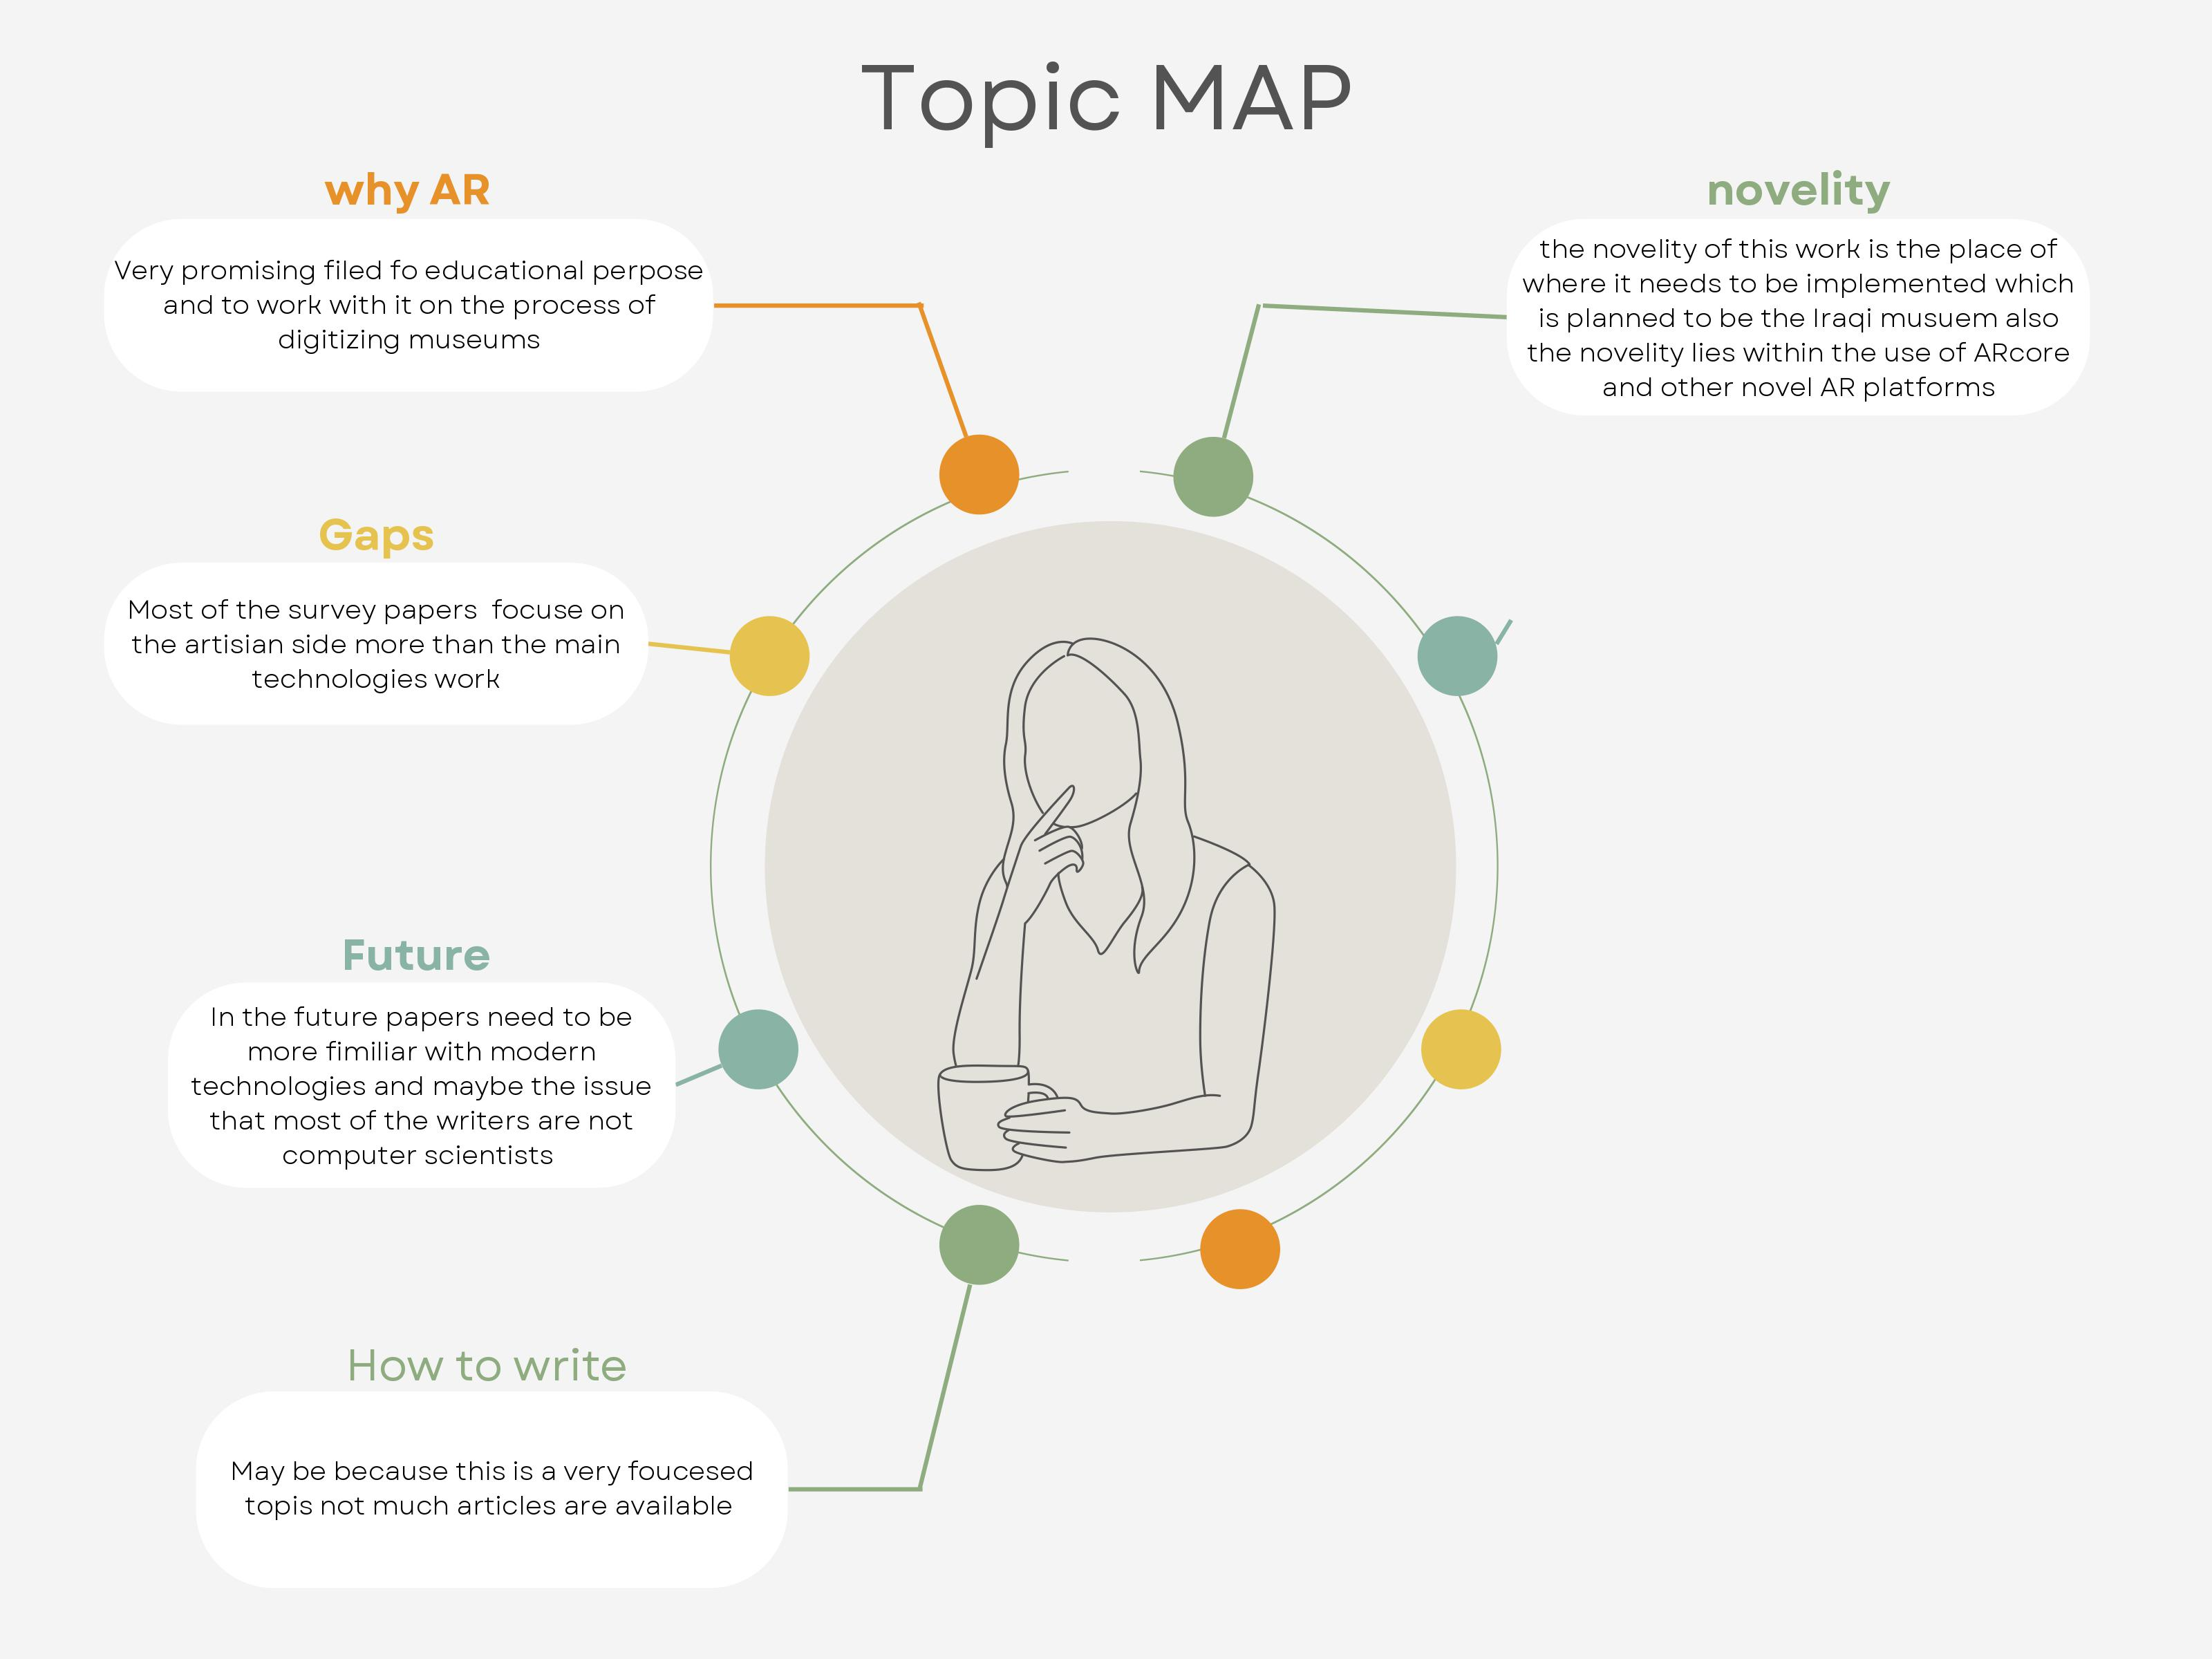
\includegraphics[width=100mm]{Topic MAP.jpg}

\label{fig:method}
\end{figure}
\medskip
\bibliographystyle{plain}


\bibliography{sample}
\end{document}
